\documentclass[12pt,a4paper,oneside]{report}
\usepackage[margin=2.5cm]{geometry}
\usepackage[T1]{fontenc}
\usepackage{lmodern}
\usepackage{microtype}
\usepackage{adjustbox}
\usepackage{graphicx,booktabs,amsmath,amssymb,xcolor,tikz,float,caption,subcaption,enumitem,array,tabularx}
\usepackage{setspace}
\usepackage{fancyhdr}
\usepackage{titlesec}
\usepackage{tcolorbox}
\usepackage[hidelinks]{hyperref}
\usetikzlibrary{arrows.meta,positioning}
\graphicspath{{../results/figures/}{./}}
\setlist{itemsep=2pt,topsep=4pt}
\captionsetup{font=small,labelfont=bf}
\onehalfspacing
\setlength{\parindent}{1.5em}
\setlength{\parskip}{3pt}
\newcommand{\fit}[1]{\begin{adjustbox}{max width=\linewidth}\input{generated/#1.tex}\end{adjustbox}}
\newcolumntype{Y}{>{\raggedright\arraybackslash}X}

\titleformat{\chapter}[display]{\normalfont\Large\bfseries}{\large Chapter \thechapter}{4pt}{\LARGE}
\titlespacing*{\chapter}{0pt}{-20pt}{18pt}
\titleformat{\section}{\normalfont\large\bfseries}{\thesection}{0.7em}{}
\titleformat{\subsection}{\normalfont\normalsize\bfseries}{\thesubsection}{0.7em}{}

\pagestyle{fancy}
\fancyhf{}
\fancyhead[L]{\small UCS760 -- Reinforcement Learning}
\fancyhead[R]{\small EdgeBot: Robust Safety Shield for Edge RL}
\fancyfoot[C]{\thepage}
\renewcommand{\headrulewidth}{0.4pt}
\fancypagestyle{plain}{\fancyhf{}\fancyfoot[C]{\thepage}\renewcommand{\headrulewidth}{0pt}}
\renewcommand{\bibname}{References}

\tcbset{novelty/.style={colback=orange!6,colframe=orange!70!black,boxrule=0.8pt,arc=2pt,left=6pt,right=6pt,top=4pt,bottom=4pt}}

\begin{document}

% =====================================================================
% COVER PAGE
% =====================================================================
\begin{titlepage}
\newgeometry{margin=2.2cm}
\centering

\includegraphics[width=0.82\linewidth]{thapar_logo.png}\par
\vspace{1.6cm}
{\large\scshape Project Report\par}
\vspace{0.9cm}
{\Huge\bfseries EdgeBot\par}
\vspace{0.5cm}
{\Large A Robust, Map-Free Lidar Safety Shield for\\[3pt] Quantised Reinforcement Learning Navigation\\[3pt] in a Voice-Commanded Warehouse Robot\par}
\vspace{1.4cm}
{\large Course: \textbf{UCS760 -- Reinforcement Learning}\par}
\vspace{2.2cm}
\begin{minipage}[t]{0.47\linewidth}
\raggedright
{\large Submitted by:}\\[6pt]
{\large\bfseries Mehul Khanna}\\[2pt]
{\large Roll No.\ 10232334}
\end{minipage}\hfill
\begin{minipage}[t]{0.47\linewidth}
\raggedleft
{\large Submitted to:}\\[6pt]
{\large\bfseries Dr.\ Himika Sharma}\\[2pt]
{\large Assistant Professor}
\end{minipage}
\vfill
{\large Department of Computer Science and Engineering\par}
{\large Thapar Institute of Engineering and Technology, Patiala\par}
\vspace{0.3cm}
{\large November 2026\par}
\restoregeometry
\end{titlepage}

% =====================================================================
% FRONT MATTER
% =====================================================================
\pagenumbering{roman}
\chapter*{Declaration}
\addcontentsline{toc}{chapter}{Declaration}
I hereby declare that the project report entitled \emph{``EdgeBot: A Robust, Map-Free Lidar Safety Shield for
Quantised Reinforcement Learning Navigation in a Voice-Commanded Warehouse Robot''}, submitted for the course
UCS760 (Reinforcement Learning) at Thapar Institute of Engineering and Technology, Patiala, is a record of my own
work carried out under the guidance of Dr.\ Himika Sharma. All existing methods, models, libraries and published
results used in this work have been acknowledged and cited.

\vspace{2cm}
\noindent Mehul Khanna\\
Roll No.\ 10232334\\
Date: \rule{4cm}{0.4pt}

\chapter*{Acknowledgement}
\addcontentsline{toc}{chapter}{Acknowledgement}
I am grateful to Dr.\ Himika Sharma, Assistant Professor, Department of Computer Science and Engineering, for
teaching UCS760 and for her guidance throughout the semester. The ideas used in this project, from Markov decision
processes and temporal-difference learning to deep Q-networks and policy-gradient methods, were first introduced in
her lectures and laboratory sessions.

I also thank the Department of Computer Science and Engineering, TIET, for the facilities provided, and the
developers of the open-source tools used in this work: PyTorch, Gymnasium, Hugging Face Transformers, ONNX Runtime,
faster-whisper and Piper.

\vspace{2cm}
\noindent Mehul Khanna\\
Roll No.\ 10232334

\chapter*{Abstract}
\addcontentsline{toc}{chapter}{Abstract}
Reinforcement learning (RL) policies for robot navigation are increasingly compressed to 8-bit integers (INT8) so
that they can run on low-cost edge hardware, and recent studies show that this compression can silently change the
actions a policy takes. At the same time, \emph{safety shields}, filters that block unsafe actions, have become a
standard tool for safe RL, but most of them need a map or a formal model of the world, or are themselves trained
neural networks, and they are usually evaluated on full-precision policies with clean sensors.

The main contribution of this project is a \textbf{robust, map-free and training-free lidar safety shield} that sits
between any learned navigation policy and the motors. At every control step it predicts the robot's motion for the
next 0.5\,s from its own kinematics, checks the predicted path against the current lidar scan, and replaces an
unsafe action with the closest safe one. A three-beam median filter makes the shield robust to faulty lidar readings.
The shield needs no map, no retraining and no extra network, costs about 0.15\,ms per decision, and works unchanged
for PPO and DQN policies in both FP32 and INT8 form.

The shield is evaluated inside \emph{EdgeBot}, a complete simulated warehouse robot that is commanded by voice
(Whisper speech recognition, a distilled BERT-style language model, Piper speech synthesis), plans routes with A*,
drives with a PPO policy trained on randomly generated warehouses, and picks objects with a 3-joint arm. On 300
warehouse layouts never seen during training, the PPO policy reaches the goal in 96.0\% of episodes; the shield
reduces its collision rate from 2.0\% to \textbf{0.0\%} without lowering success, and does the same for every INT8
policy tested. Under lidar corruption reproduced from a 2025 study, a naive shield freezes the robot (3.0\% success),
while the robust shield keeps 93.7--95.0\% success with 0--1\% collisions, which is better than retraining the policy
with domain randomisation (89.3\% success, 7.0\% collisions). The project also reproduces the classical tabular RL
results (dynamic programming, Monte Carlo, SARSA, Q-learning) and compares DQN with PPO.

\tableofcontents
\listoffigures
\listoftables
\clearpage
\pagenumbering{arabic}

% =====================================================================
\chapter{Introduction}
\label{ch:intro}

\section{Motivation}
Warehouses are one of the fastest-growing application areas of mobile robots. A warehouse robot must do three
things well: move among shelves, pallets and people without colliding with anything, pick up and place items
accurately, and understand instructions given by workers who are not programmers. The layout of a warehouse
changes every day as goods arrive and leave, so a fixed, hand-written path follower is not enough; the robot has to
\emph{react} to whatever its sensors see. Deep reinforcement learning (DRL) is well suited to this, because the
robot learns a reactive driving policy from experience instead of from hand-written rules.

A recent survey of DRL for mobile-robot navigation in dynamic environments (Zhu et al., \emph{Sensors}, 2025)
reviewed the literature published between 2021 and 2024 and found that lidar and vision are the dominant sensors,
that only about half of the 22 representative studies it analysed in detail were validated on physical robots, and
that \textbf{safety}, \textbf{sim-to-real transfer} and \textbf{robustness to sensor noise} are among the main open
problems~\cite{zhu2025survey}. A second survey on sim-to-real methods in RL (2025) reaches a similar
conclusion~\cite{sim2realsurvey2025}. These two problems are made harder when the policy is deployed on a small
on-board computer: to fit and run fast, the policy is quantised to INT8, and quantisation is known to change the
actions of RL policies~\cite{quarl,quantprune2024,quantctrl2025}.

\section{Problem statement}
\emph{Design and evaluate a voice-commanded warehouse robot whose navigation is learned with reinforcement learning,
and make the learned navigation policy \textbf{provably cautious at run time}, so that it does not collide even when
the policy is compressed to INT8 for edge hardware and even when the lidar returns faulty readings, without
requiring a map, retraining or an additional neural network.}

\section{The novelty of this project}
\begin{tcolorbox}[novelty,title=\textbf{Novelty in one paragraph}]
This project proposes a \textbf{robust, map-free, training-free kinematic lidar safety shield} for learned navigation
policies running on edge devices. The shield predicts the robot's path from its own motion model, checks it against
the live lidar scan, and replaces unsafe actions with the nearest safe action. A median filter over neighbouring
beams makes it robust to spurious lidar returns. It is evaluated side by side on \textbf{full-precision and INT8
policies}, under \textbf{clean and corrupted lidar}, inside a complete voice-commanded robot. To the best of my
knowledge, existing shields either need a map or a formal model, are themselves learned networks, or are tested on
full-precision policies only (Chapter~\ref{ch:lit}).
\end{tcolorbox}

\section{Contributions}
\begin{enumerate}
\item \textbf{(Main) A map-free, training-free lidar safety shield} that removes collisions for PPO and DQN policies
in both FP32 and INT8 form on 300 unseen layouts (2.0\%$\to$0.0\% for the deployed PPO).
\item \textbf{(Main) A robust variant of the shield} that survives lidar corruption taken from a 2025
study~\cite{omni2025}: the naive shield freezes the robot (3.0\% success) while the robust shield keeps 93.7\%
(FP32) and 95.0\% (INT8) success with at most 1.0\% collisions.
\item \textbf{A direct comparison with the standard alternative from the literature}, retraining the policy with
domain randomisation, which performs worse (89.3\% success, 7.0\% collisions) and costs 5 million extra training
steps, whereas the shield needs no training.
\item \textbf{A complete RL pipeline} built from scratch: a warehouse grid MDP solved with dynamic programming,
Monte Carlo and TD methods; a Gymnasium-style continuous navigation environment; DQN and PPO agents; and a test of
the SimBa network design from ICLR 2025~\cite{simba2025}.
\item \textbf{A working voice-commanded robot} that integrates the shielded policy with A* planning, an inverse
kinematics arm, a distilled language model and speech, all exported to ONNX/INT8.
\end{enumerate}

\section{Organisation of the report}
Chapter~\ref{ch:lit} surveys the related work and identifies the research gap. Chapter~\ref{ch:bg} summarises the
RL theory used. Chapter~\ref{ch:design} describes the system design and justifies each design choice.
Chapter~\ref{ch:rl} presents the RL experiments that produce the navigation policy. Chapter~\ref{ch:novel}, the
core of the report, describes the proposed safety shield, its robust variant, and its evaluation and comparison
with existing approaches. Chapter~\ref{ch:recent} reports an additional recent technique (SimBa).
Chapter~\ref{ch:support} covers the supporting modules, Chapter~\ref{ch:demo} the integrated demonstration,
Chapter~\ref{ch:discussion} the discussion, and Chapter~\ref{ch:conclusion} the conclusion. Appendix~\ref{app:qa}
lists anticipated questions and answers, and Appendix~\ref{app:repro} explains how to reproduce the results.

% =====================================================================
\chapter{Literature Survey and Research Gap}
\label{ch:lit}

\section{Survey data: DRL for mobile-robot navigation}
Table~\ref{tab:survey} summarises the key findings of the 2025 review by Zhu et al.~\cite{zhu2025survey}, which is
used here as the reference survey for the state of the field.

\begin{table}[H]
\centering\small
\caption{Findings of the survey ``Deep Reinforcement Learning of Mobile Robot Navigation in Dynamic Environment:
A Review'' (Zhu et al., \emph{Sensors} 25(11):3394, 2025).}
\label{tab:survey}
\begin{tabularx}{\linewidth}{lY}
\toprule
Aspect & Finding of the survey \\
\midrule
Period reviewed & Literature published between 2021 and 2024. \\
Studies analysed in detail & 22 representative studies (Table 5 of the survey). \\
Real-robot validation & Approximately 50\% of these studies ran physical experiments; the rest were simulation only. \\
Sensors & Lidar and vision dominate; multimodal fusion improves robustness. \\
Algorithms & Value-based (DQN, Double DQN, Dueling DQN), policy-based (PPO, TRPO) and actor-critic hybrids (DDPG, TD3, SAC, A3C). \\
Open challenges & (1) adaptability in dynamic environments, (2) multimodal fusion under sensor noise and delays,
(3) multi-robot collaboration, (4) sim-to-real transfer, (5) safety and explainability, (6) cross-domain applications. \\
\bottomrule
\end{tabularx}
\end{table}

Two of the six open challenges, \textbf{safety} and \textbf{robustness to sensor noise}, are exactly what the
proposed shield addresses. The survey also notes that ``sensor noise, delays, or asynchronous updates between
modalities can lead to policy divergence'' and that ``most current DRL algorithms operate as black-box systems''.
A shield is a transparent, rule-based layer on top of a black-box policy, so it directly answers the second point.

\section{Safe reinforcement learning with shields}
Alshiekh et al.~\cite{alshiekh} introduced \emph{shielding}: a component that monitors the actions of an RL agent and
corrects any action that would violate a safety specification. Their shield is synthesised from a formal model of
the environment. Later work extends shields to continuous spaces: realizable continuous-space shields
(2024)~\cite{realizable2024} are evaluated with PPO on lidar navigation and rely on a model of the system dynamics.
REASAN (2025)~\cite{reasan2025} trains a reactive safety policy for legged robots that uses a single lidar, i.e.\ the
safety layer is itself a learned network. Lightweight safe RL for UAV navigation (2026)~\cite{uavsafe2026} studies
safety under sparse lidar observations.

\section{Quantised RL policies on edge hardware}
QuaRL (2022)~\cite{quarl} showed that quantising RL policies reduces cost but can change their behaviour. A 2024
study~\cite{quantprune2024} measured the impact of quantisation and pruning on deep RL models, and a 2025
paper~\cite{quantctrl2025} learns quantised continuous controllers for integer hardware. A 2026
survey~\cite{edgesurvey2026} lists the deployment constraints of running learned models on robots at the edge.
These works improve or measure the policy itself; they do not add a run-time safety layer.

\section{Sim-to-real transfer and sensor corruption}
Recent sim-to-real work deliberately corrupts sensors in simulation so that policies transfer to real
robots~\cite{sim2real2025,sim2realsurvey2025,navrlpp2026}. Omni-Perception (2025)~\cite{omni2025} trains with 10\% of
lidar points replaced by spurious short readings in $[0,0.3]$\,m and 10\% distance noise. This corruption model is
reused in this project to stress-test the shield (Section~\ref{sec:robust}).

\section{Research gap}
Table~\ref{tab:gap} compares the properties of the closest existing approaches with the proposed shield. The
comparison is based on the problem each work targets, as described in its paper.

\begin{table}[H]
\centering\small
\caption{Comparison of the proposed shield with related work.}
\label{tab:gap}
\begin{tabularx}{\linewidth}{lYcccc}
\toprule
Work & Main idea & \rotatebox{90}{No map/model} & \rotatebox{90}{No training} & \rotatebox{90}{Tested on INT8} & \rotatebox{90}{Sensor faults} \\
\midrule
Alshiekh et al.\ 2018~\cite{alshiekh} & Shield from formal model & -- & \checkmark & -- & -- \\
Realizable shields 2024~\cite{realizable2024} & Continuous shield from dynamics model & -- & \checkmark & -- & -- \\
REASAN 2025~\cite{reasan2025} & Learned lidar safety policy & \checkmark & -- & -- & -- \\
QuaRL 2022~\cite{quarl}, 2024~\cite{quantprune2024} & Measure/limit quantisation effects & n/a & n/a & \checkmark & -- \\
Domain randomisation~\cite{omni2025,sim2real2025} & Retrain with sensor noise & \checkmark & -- & -- & \checkmark \\
\midrule
\textbf{This project} & \textbf{Kinematic lidar shield + median filter} & \checkmark & \checkmark & \checkmark & \checkmark \\
\bottomrule
\end{tabularx}
\end{table}

\begin{tcolorbox}[novelty,title=\textbf{Research gap addressed}]
No single approach above is at the same time (i)~map-free, (ii)~training-free, (iii)~evaluated on quantised edge
policies and (iv)~robust to faulty lidar readings. The proposed shield satisfies all four, and it is measured side by
side against the strongest training-based alternative (domain randomisation) on the same 300 test layouts.
\end{tcolorbox}

% =====================================================================
\chapter{Background}
\label{ch:bg}

\section{Markov decision processes}
An RL problem is modelled as a Markov decision process (MDP) $(S,A,P,R,\gamma)$. At each step the agent observes a
state $s$, takes an action $a$, receives a reward $r$ and moves to a new state $s'$ with probability $P(s'\mid s,a)$.
The goal is a policy $\pi(a\mid s)$ that maximises the expected discounted return
$G_t=\sum_{k\ge0}\gamma^k R_{t+k+1}$. The optimal action-value function satisfies the Bellman optimality equation
\[ q_*(s,a)=\sum_{s',r}p(s',r\mid s,a)\big[r+\gamma\max_{a'}q_*(s',a')\big]. \]

\section{Dynamic programming, Monte Carlo and TD learning}
If the model is known, \emph{value iteration} and \emph{policy iteration} compute the optimal policy exactly.
Without a model, the agent learns from experience. \emph{Monte Carlo} methods wait until the end of an episode and
update towards the observed return; \emph{temporal-difference} (TD) methods update after every step towards
$r+\gamma V(s')$. SARSA (on-policy) and Q-learning (off-policy) are the two basic TD control methods~\cite{sutton}.

\section{Deep Q-networks}
For large or continuous state spaces a neural network approximates the value function. DQN~\cite{dqn} uses an
experience replay buffer and a target network for stability; Double DQN~\cite{ddqn} reduces over-estimation by
selecting the next action with the online network and evaluating it with the target network.

\section{Proximal policy optimisation}
PPO~\cite{ppo} is an actor-critic policy-gradient method. The actor outputs a distribution over actions and the
critic estimates $V(s)$. Advantages are estimated with GAE~\cite{gae}, and the clipped objective
\[ L^{\text{CLIP}}(\theta)=\mathbb{E}_t\Big[\min\big(\rho_t\hat A_t,\ \mathrm{clip}(\rho_t,1-\epsilon,1+\epsilon)\hat A_t\big)\Big],
\qquad \rho_t=\frac{\pi_\theta(a_t\mid s_t)}{\pi_{\theta_{\text{old}}}(a_t\mid s_t)}, \]
limits how far one update can move the policy, which makes training stable.

% =====================================================================
\chapter{System Design}
\label{ch:design}

\section{Architecture}
Figure~\ref{fig:arch} shows the complete system. The safety shield, the novelty of this project, sits between the
learned policy and the motors, so every action the robot executes has passed through it.

\begin{figure}[H]
\centering
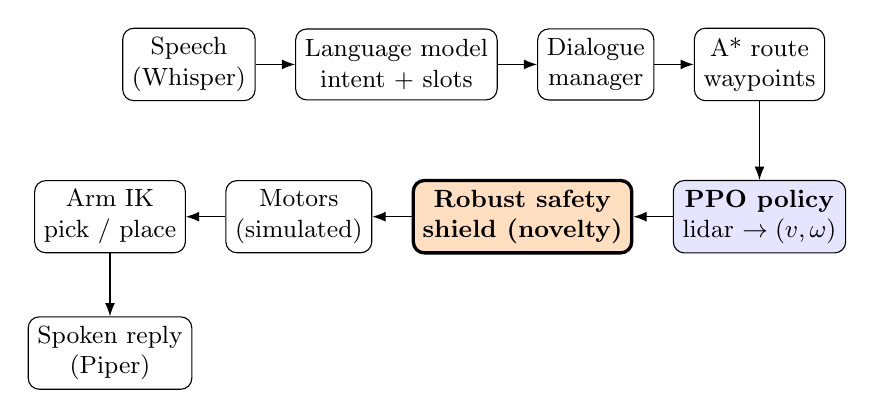
\begin{tikzpicture}[node distance=5mm, every node/.style={draw, rounded corners, align=center, font=\small, minimum height=9mm}]
\node (asr) {Speech\\(Whisper)};
\node (nlu) [right=of asr] {Language model\\intent + slots};
\node (dm) [right=of nlu] {Dialogue\\manager};
\node (plan) [right=of dm] {A* route\\waypoints};
\node (rl) [below=10mm of plan, fill=blue!10] {\textbf{PPO policy}\\lidar $\to(v,\omega)$};
\node (sh) [left=of rl, fill=orange!25, very thick] {\textbf{Robust safety}\\\textbf{shield (novelty)}};
\node (mot) [left=of sh] {Motors\\(simulated)};
\node (arm) [left=of mot] {Arm IK\\pick / place};
\node (tts) [below=8mm of arm] {Spoken reply\\(Piper)};
\draw[-{Latex}] (asr)--(nlu); \draw[-{Latex}] (nlu)--(dm); \draw[-{Latex}] (dm)--(plan); \draw[-{Latex}] (plan)--(rl);
\draw[-{Latex}] (rl)--(sh); \draw[-{Latex}] (sh)--(mot); \draw[-{Latex}] (mot)--(arm); \draw[-{Latex}] (arm)--(tts);
\end{tikzpicture}
\caption{EdgeBot architecture. Every action of the learned policy passes through the safety shield.}
\label{fig:arch}
\end{figure}

\section{Data flow for one command}
For the command \emph{``move the red box from shelf A to the conveyor''}: Whisper converts speech to text; the
language model extracts the intent (pick and place) and the slots (colour = red, object = box, source = shelf A,
destination = conveyor); the dialogue manager checks the request against the inventory and asks for missing
information; A* plans a route; the PPO policy drives between waypoints ten times per second while the shield checks
each action; the arm picks and places the box using inverse kinematics; and Piper speaks the reply.

\section{Justification of design choices}
\begin{table}[H]
\centering\small
\caption{Design choices and their justification.}
\label{tab:choices}
\begin{tabularx}{\linewidth}{lYY}
\toprule
Component & Choice & Justification \\
\midrule
Training world & Own 2-D simulator, Gymnasium API & RL needs millions of trials and crashes; the simulator runs 5M steps in about 25 minutes and allows repeatable tests on identical layouts. \\
Layouts & New random warehouse every episode & Prevents memorisation; forces the policy to generalise. \\
Navigation learner & PPO with continuous actions & Highest success (96.0\%), smooth control, stable updates, tiny network (Chapter~\ref{ch:rl}). \\
Global planning & A* + learned local policy & A purely reactive policy can be trapped behind long shelves; A* gives waypoints, RL handles obstacles. \\
Safety & Kinematic lidar shield (novelty) & Needs no map, no training and no extra network; protects FP32 and INT8 policies (Chapter~\ref{ch:novel}). \\
Robustness & Three-beam median filter & Removes isolated fake readings while keeping real obstacles, which cover adjacent beams. \\
Arm & Closed-form inverse kinematics & The geometry is known exactly; IK is exact, whereas the RL reaching agent has 5\,mm error. \\
Language & Distilled BERT-style model & 135$\times$ smaller than DistilBERT at 97.6\% accuracy; fits on an edge device. \\
Deployment & ONNX + INT8 & Portable format accepted by TensorRT on Jetson; 3--4$\times$ smaller models. \\
\bottomrule
\end{tabularx}
\end{table}

% =====================================================================
\chapter{Reinforcement Learning Experiments}
\label{ch:rl}

\section{Tabular RL on a warehouse grid}
A $5\times10$ grid models the warehouse. The robot starts at the loading bay and must reach the packing station;
each step costs $-1$, and an oil spill along the shortest route costs $-100$ and returns the robot to the start,
which is the warehouse analogue of the Cliff Walking problem~\cite{sutton}. A slippery variant moves the robot
sideways with a given probability. Value iteration and policy iteration produce the same value function
(Table~\ref{tab:dp}, Figure~\ref{fig:dp}).

\begin{table}[H]\centering\small\caption{Dynamic programming results.}\label{tab:dp}\fit{tab_dp}\end{table}
\begin{figure}[H]\centering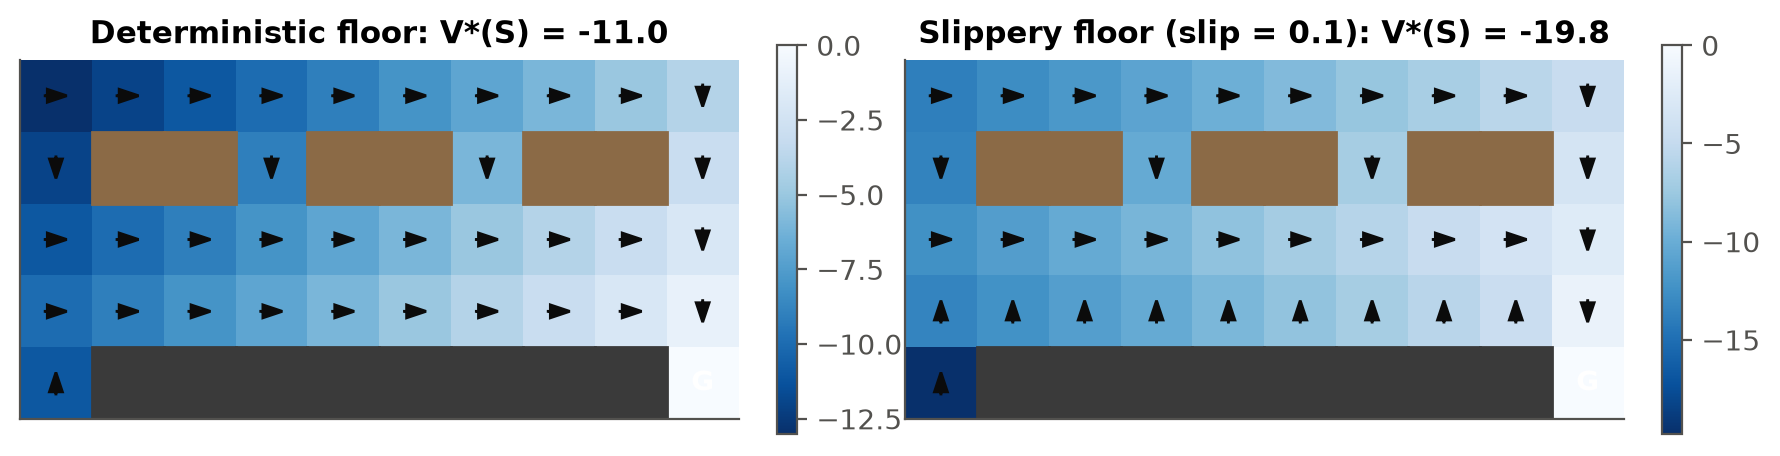
\includegraphics[width=0.95\linewidth]{dp_value_policy.png}
\caption{Optimal value function and policy on the deterministic and the slippery floor.}\label{fig:dp}\end{figure}

Model-free methods were run with 20 random seeds and $\varepsilon=0.1$ (Table~\ref{tab:control},
Figure~\ref{fig:tab}). Q-learning learns the optimal 11-step path beside the spill but falls into the spill during
exploration, so its online return is low. SARSA accounts for its own exploration and learns a safer 17-step path with
a higher online return. Expected SARSA gives the best online return, and Monte Carlo is the slowest because the
$-100$ penalties make its returns highly variable.

\begin{table}[H]\centering\small\caption{Model-free control (20 runs, 500 episodes; Monte Carlo 2000).}\label{tab:control}\fit{tab_control}\end{table}
\begin{figure}[H]\centering
\begin{subfigure}{0.6\linewidth}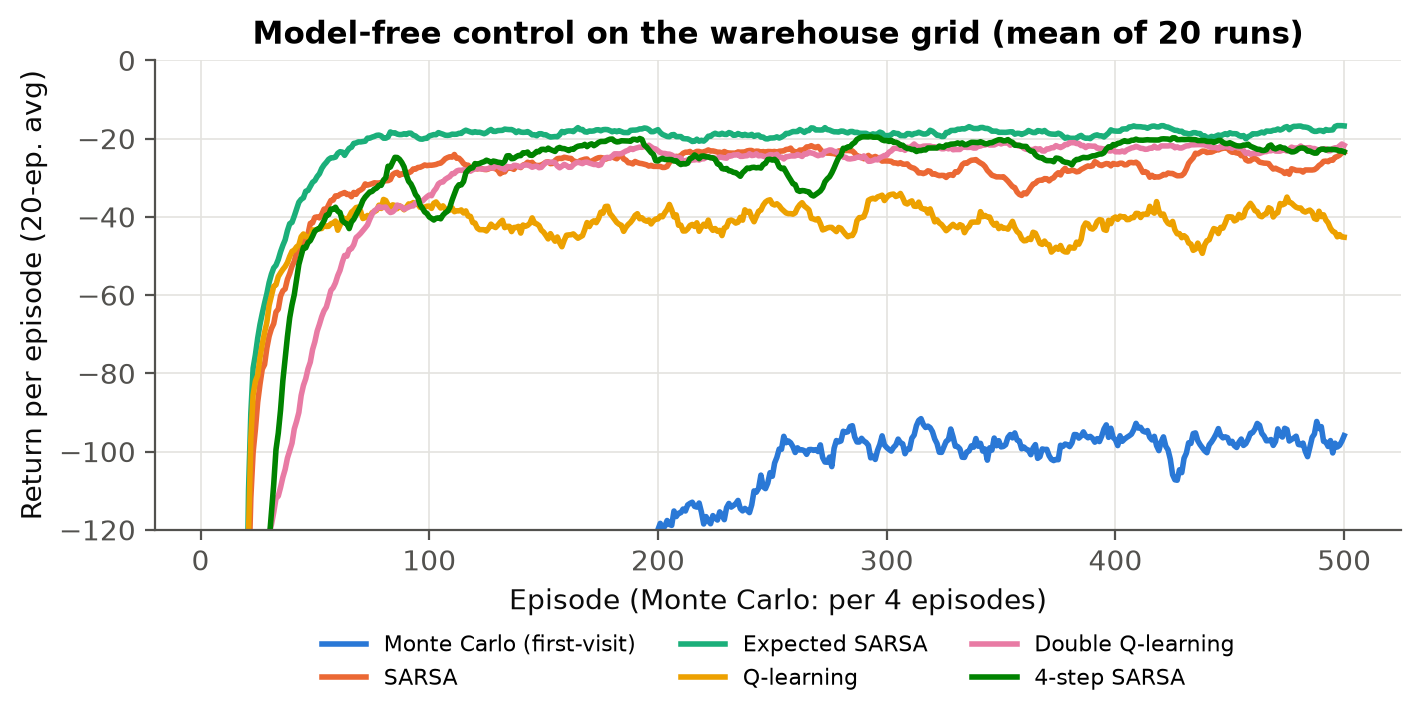
\includegraphics[width=\linewidth]{tabular_learning_curves.png}\end{subfigure}
\begin{subfigure}{0.38\linewidth}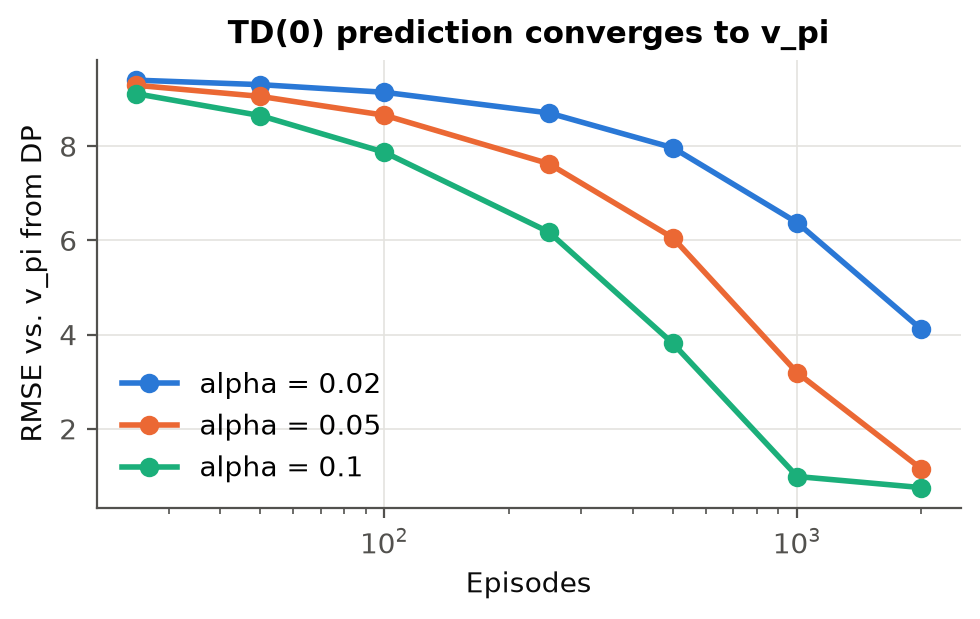
\includegraphics[width=\linewidth]{td0_prediction.png}\end{subfigure}
\caption{Left: learning curves of the tabular methods. Right: TD(0) prediction error versus the exact values.}\label{fig:tab}\end{figure}

\section{Continuous navigation environment}
The robot is a disc of radius 0.12\,m with differential-drive (unicycle) kinematics at 10\,Hz. Its \textbf{state}
has 29 values: 24 lidar distances over 360$^\circ$, the distance and direction to the goal, and the previous action.
Its \textbf{action} is a forward speed $v\in[0,0.5]$\,m/s and a turn rate $\omega\in[-2,2]$\,rad/s (or 5 discrete
motions for DQN). The \textbf{reward} is $3\times$ the progress towards the goal, $-0.01$ per step, small penalties
for passing close to obstacles and for jerky turning, $+10$ for reaching the goal and $-10$ for a collision, which ends
the episode. Each episode generates a new warehouse with up to 4 shelves and 1--7 round obstacles. A second
observation mode provides a $64\times64$ egocentric image for vision-based RL.

\section{Training and results}
PPO uses separate $128\times128$ actor and critic networks, 16 parallel environments, GAE ($\lambda=0.95$), clip
$0.2$ and 5 million steps. DQN uses Double DQN with a dueling head, a replay buffer, a target network and
$\varepsilon$ decaying from 1.0 to 0.03. All policies are tested on 300 layouts generated from seeds never used in
training (Table~\ref{tab:nav}, Figures~\ref{fig:navcurves}--\ref{fig:traj}).

\begin{table}[H]\centering\small\caption{Navigation results on 300 unseen layouts.}\label{tab:nav}\fit{tab_nav}\end{table}
\begin{figure}[H]\centering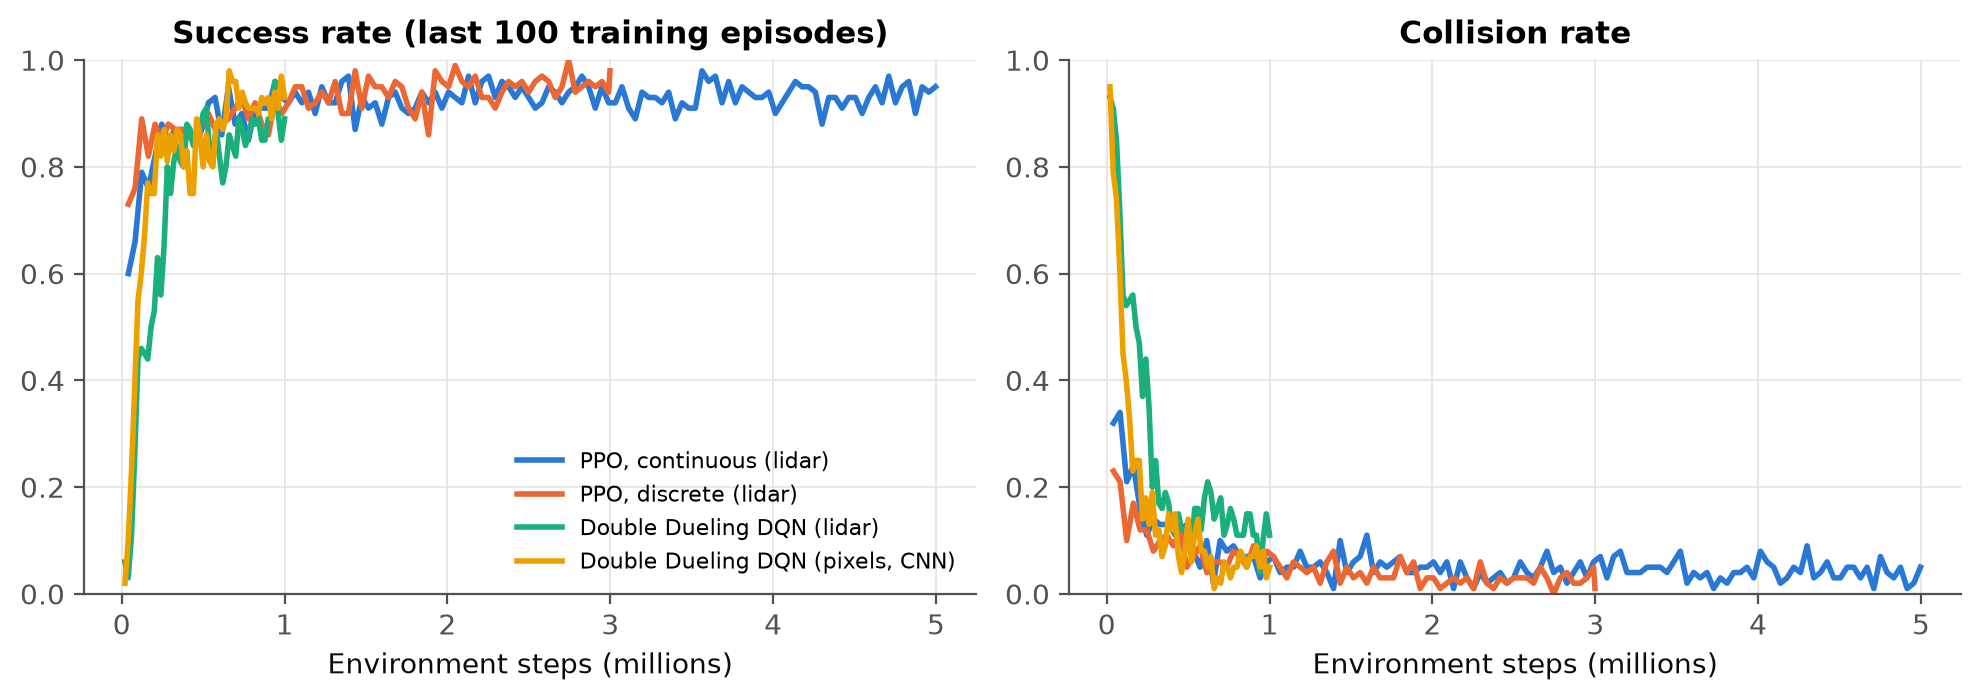
\includegraphics[width=\linewidth]{nav_learning_curves.png}
\caption{Training curves (rolling mean over the last 100 episodes).}\label{fig:navcurves}\end{figure}
\begin{figure}[H]\centering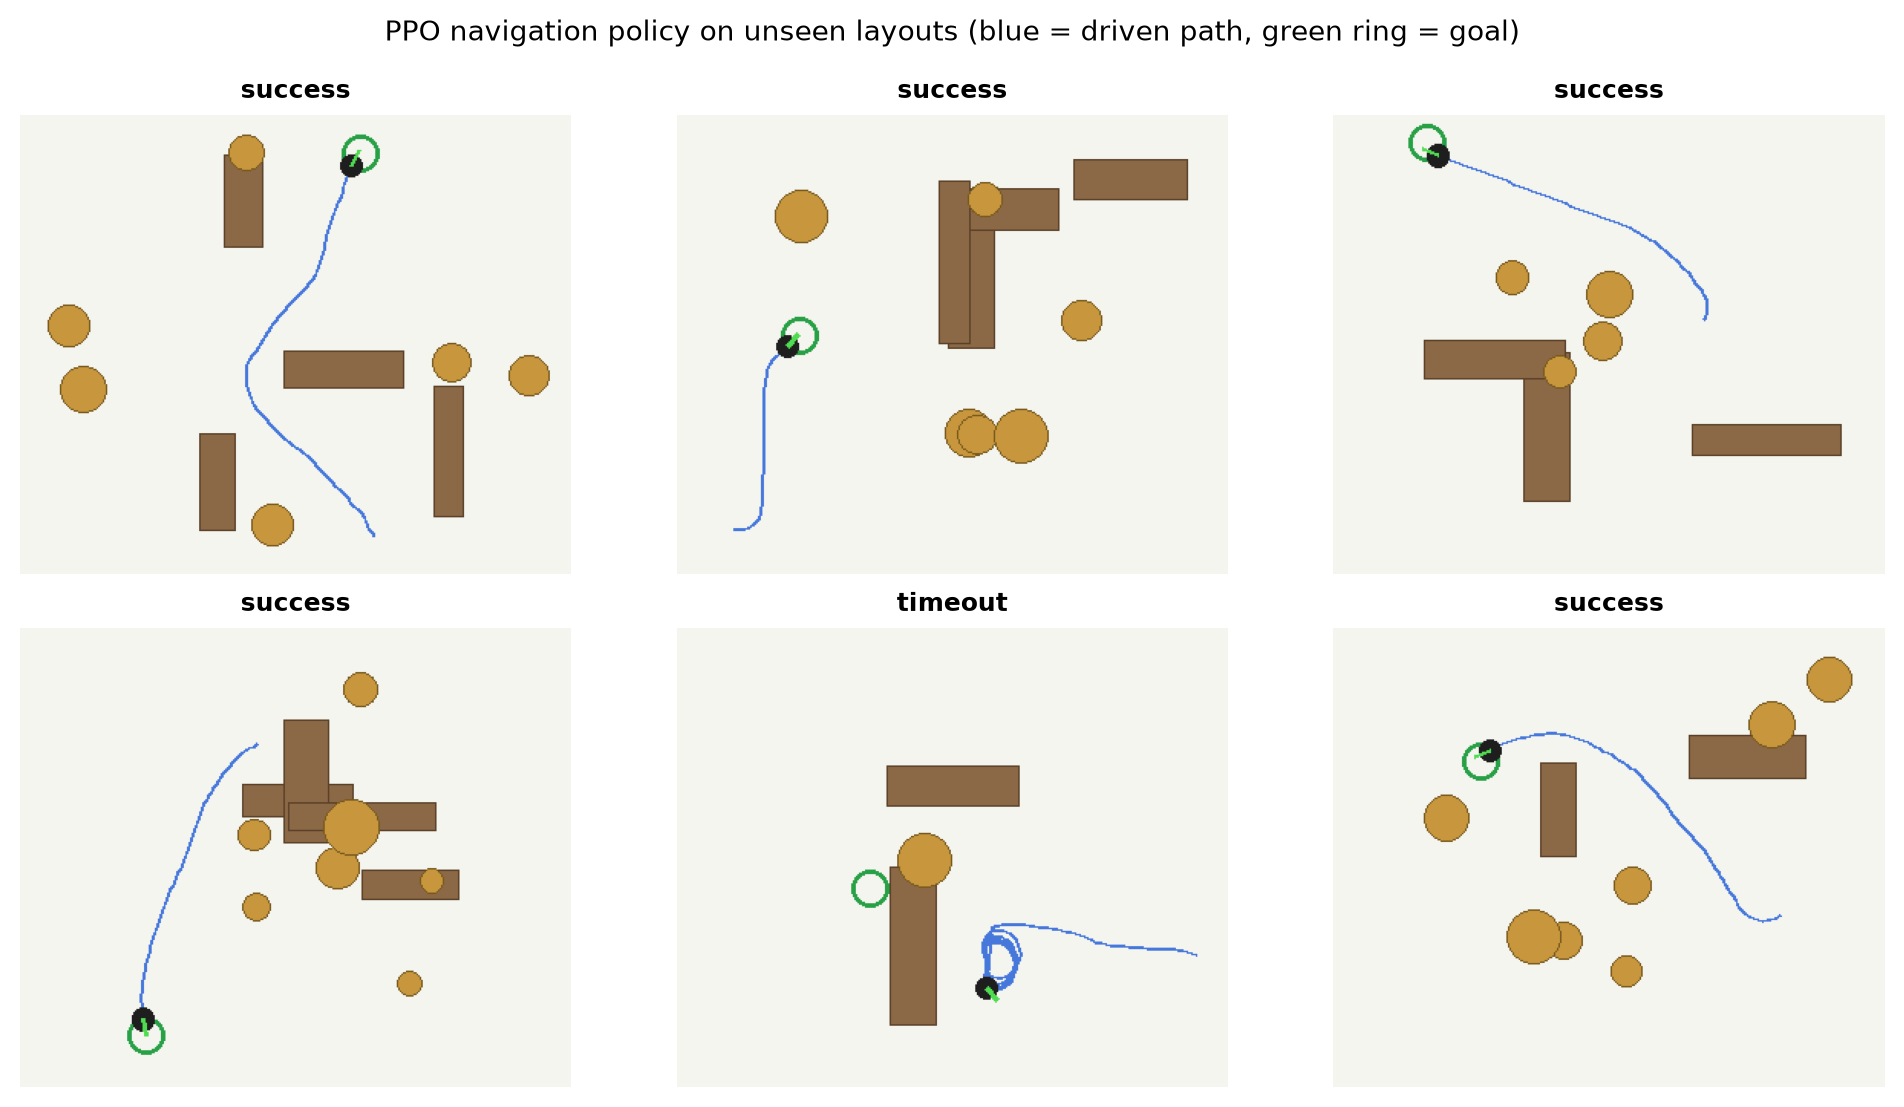
\includegraphics[width=0.85\linewidth]{nav_trajectories.png}
\caption{Paths of the PPO policy on unseen layouts.}\label{fig:traj}\end{figure}

PPO with continuous actions is selected for deployment: it has the highest success rate, smooth continuous control
and a network of only 21\,k parameters. Even this policy, however, collides in 2.0\% of episodes, and its INT8
version collides in 3.0\%. In a real warehouse, one collision in every fifty trips is not acceptable. This residual
risk is the motivation for the novelty described next.

% =====================================================================
\chapter{Novelty: A Robust, Map-Free Lidar Safety Shield}
\label{ch:novel}

\begin{tcolorbox}[novelty,title=\textbf{Key idea}]
Do not trust the learned policy blindly. Before each action reaches the motors, predict where the robot will be in
the next 0.5\,s using only its own motion equations and the current lidar scan. If the predicted path comes too
close to any obstacle, replace the action with the nearest safe one. Filter the lidar first so that a single faulty
beam cannot trigger a false alarm.
\end{tcolorbox}

\section{Why a shield is needed}
A neural policy is trained to maximise expected reward, not to guarantee safety. Three effects leave a residual
collision risk: (i)~the policy is never perfect on unseen layouts (2.0\% collisions for the deployed PPO);
(ii)~INT8 quantisation perturbs the network's weights and can change its actions~\cite{quarl,quantprune2024}; and
(iii)~real lidars return noisy and spurious readings~\cite{omni2025}. Retraining cannot remove these effects
entirely and must be repeated for every new policy. A run-time shield addresses all three at once, for any policy.

\section{The shield algorithm}
At every control step (every 0.1\,s):
\begin{enumerate}
\item The policy (PPO or DQN, FP32 or INT8) proposes an action $(v,\omega)$.
\item \textbf{Filtering (robust variant).} Each lidar distance $r_i$ is replaced by the median of
$\{r_{i-1},r_i,r_{i+1}\}$ over the circular scan.
\item \textbf{Obstacle points.} Each beam that returns a distance shorter than the maximum range is converted into a
point $(r_i\cos\alpha_i,\ r_i\sin\alpha_i)$ in the robot frame.
\item \textbf{Prediction.} The robot's motion is simulated for $H=5$ steps (0.5\,s) with the unicycle model while
holding $(v,\omega)$.
\item \textbf{Check.} If any predicted position is closer than the robot radius plus a 4\,cm margin to any obstacle
point, the action is unsafe.
\item \textbf{Correction.} An unsafe action is replaced by the candidate (forward, gentle turns, slow, spin) that is
closest to the proposed action and passes the check. A pure spin does not move the robot, so a safe action always
exists.
\end{enumerate}
The implementation (\texttt{edgebot/rl/shield.py}) has 73 lines and uses only the lidar scan and the robot's
kinematics.

\section{Why it works: justification}
\begin{itemize}
\item \textbf{Map-free.} The lidar scan already contains every nearby obstacle, including ones that are not on any
map (fallen boxes, people), so no map is required.
\item \textbf{Training-free.} The check uses physics (the motion equations), not learned parameters, so it does not
need data, does not need retraining when the policy changes, and cannot be degraded by quantisation.
\item \textbf{Minimal interference.} The shield replaces only unsafe actions and chooses the safe action closest to
the policy's choice, so the learned driving behaviour is kept whenever it is safe.
\item \textbf{Robust to faulty beams.} A real obstacle near the robot covers at least two neighbouring beams (beams
are 15$^\circ$ apart), whereas a spurious return is usually a single beam; the median filter removes the latter and
keeps the former.
\item \textbf{Cheap.} One check takes about 0.07\,ms (0.15\,ms with the median filter) in plain Python on one CPU
core, less than 0.2\% of the 100\,ms control period.
\end{itemize}

\section{Experiment 1: shielding FP32 and INT8 policies}
Every exported policy is evaluated on the same 300 unseen layouts with and without the shield
(\texttt{scripts/eval\_shield.py}, Table~\ref{tab:shield}).

\begin{table}[H]\centering\small\caption{Effect of the shield on FP32 and INT8 policies (300 unseen layouts).}\label{tab:shield}\fit{tab_shield}\end{table}

With the shield, collisions fall to \textbf{0.0\% for every policy}, including all INT8 versions, while the shield
intervenes on only 3.6--7.2\% of control steps. Success stays within about one percentage point of the unshielded
policy, and for INT8 PPO it rises from 95.7\% to 97.0\%. Episodes that previously ended in a crash now end in a
timeout, which is the safe way for a robot to fail. The shield prevents crashes but cannot fix a policy that is lost:
the badly quantised pixel DQN mainly fails by timing out, which is fixed by better (calibrated) quantisation
(Chapter~\ref{ch:support}).

\section{Experiment 2: robustness to faulty lidar}
\label{sec:robust}
To test the shield like a real robot, the lidar corruption of Omni-Perception (2025)~\cite{omni2025} was added to the
simulator: 10\% of the beams are replaced by spurious short readings in $[0,0.3]$\,m and every distance gets up to
$\pm$10\% noise (\texttt{scripts/eval\_robustness.py}, Table~\ref{tab:robust}, Figure~\ref{fig:robust}).

\begin{table}[H]\centering\small\caption{Robustness to lidar corruption (300 unseen layouts).}\label{tab:robust}\fit{tab_robust}\end{table}
\begin{figure}[H]\centering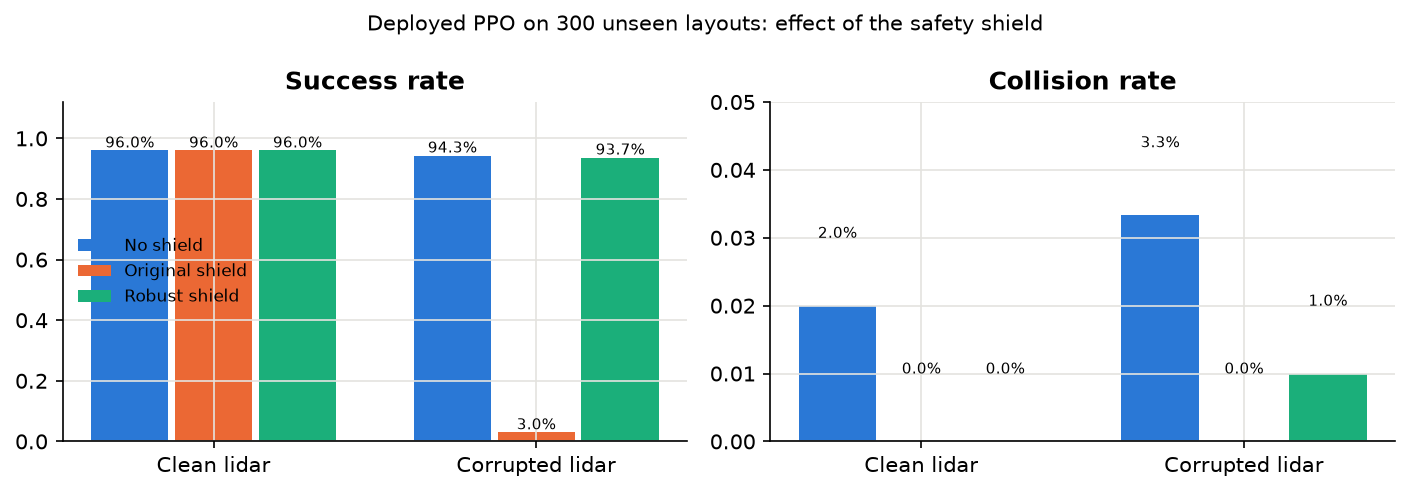
\includegraphics[width=\linewidth]{shield_robustness.png}
\caption{Deployed PPO with no shield, the original shield and the robust shield, on clean and corrupted lidar.}\label{fig:robust}\end{figure}

This experiment revealed a weakness of the first version of the shield: it trusted the fake short readings, saw
obstacles everywhere and froze the robot, so success fell to 3.0\%. The robust shield removes this failure. On
clean lidar it behaves exactly like the original (96.0\% success, 0.0\% collisions); on corrupted lidar it keeps
93.7\% success with 1.0\% collisions for the FP32 policy and 95.0\% success with 0.0\% collisions for the INT8
policy, compared with 3.0--3.3\% collisions without a shield.

\section{Experiment 3: comparison with retraining (domain randomisation)}
The standard alternative in the sim-to-real literature is to retrain the policy with the same sensor corruption
switched on~\cite{omni2025,sim2real2025}. A second PPO was trained for the same 5 million steps with the
Omni-Perception corruption. Table~\ref{tab:compare} compares the two approaches on corrupted lidar.

\begin{table}[H]
\centering\small
\caption{Proposed shield versus retraining with domain randomisation (corrupted lidar, 300 unseen layouts).}
\label{tab:compare}
\begin{adjustbox}{max width=\linewidth}
\begin{tabular}{lrrrr}
\toprule
Approach & Success & Collision & Extra training & Works for any policy \\
\midrule
Deployed PPO, no protection & 94.3\% & 3.3\% & none & -- \\
PPO retrained with domain randomisation & 89.3\% & 7.0\% & 5M steps & no \\
Deployed PPO + robust shield (FP32) & 93.7\% & 1.0\% & none & yes \\
\textbf{Deployed INT8 PPO + robust shield} & \textbf{95.0\%} & \textbf{0.0\%} & \textbf{none} & \textbf{yes} \\
\bottomrule
\end{tabular}
\end{adjustbox}
\end{table}

\begin{tcolorbox}[novelty,title=\textbf{How the novelty outperforms the existing approach}]
On the same corrupted test, the robust shield gives \textbf{higher success (95.0\% vs 89.3\%)} and \textbf{far fewer
collisions (0.0\% vs 7.0\%)} than retraining with domain randomisation, while needing \textbf{no training at all} and
working for \textbf{every policy, FP32 or INT8, PPO or DQN}. Compared with shields in the literature, it requires
neither a map nor a formal model nor a learned safety network (Table~\ref{tab:gap}).
\end{tcolorbox}

\section{Limitations of the shield}
The shield prevents collisions but does not help a policy that is lost or oscillating, so episodes that would have
crashed may end in a timeout instead. With 24 beams, very thin obstacles between two beams can be missed. The
median filter can also remove a genuine obstacle that is seen by only one beam, so the margin must be chosen with
the beam spacing in mind. Finally, the evaluation is in simulation and should be repeated on a physical robot.

% =====================================================================
\chapter{Additional Recent Technique: SimBa}
\label{ch:recent}
SimBa (ICLR 2025)~\cite{simba2025} proposes a network design for deep RL made of three parts: observation
normalisation, residual feed-forward blocks and layer normalisation. The paper reports better sample efficiency for
on-policy and off-policy algorithms. The PPO actor and critic were replaced by SimBa networks of the same width and
trained with the same settings (one seed; Table~\ref{tab:simba}, Figure~\ref{fig:simba}).

\begin{table}[H]\centering\small\caption{PPO with the plain network versus SimBa.}\label{tab:simba}\fit{tab_simba}\end{table}
\begin{figure}[H]\centering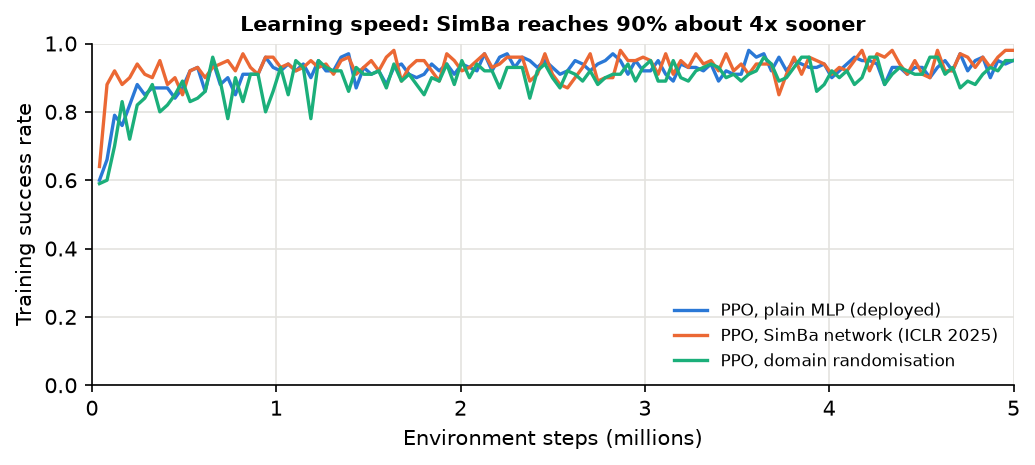
\includegraphics[width=0.85\linewidth]{recent_learning_curves.png}
\caption{Training success of the plain PPO, SimBa PPO and domain-randomised PPO.}\label{fig:simba}\end{figure}

SimBa reached 90\% training success about four times sooner (0.12M vs 0.53M steps), which agrees with the paper's
claim. Its final score after 5M steps was slightly lower (93.7\% vs 96.0\%), so the plain network remains the deployed
policy. Combined with the robust shield on corrupted lidar, SimBa PPO reached 95.0\% success with 0.7\% collisions.

% =====================================================================
\chapter{Supporting Modules}
\label{ch:support}

\section{Robot arm}
The arm has three revolute joints (links 0.35, 0.30 and 0.12\,m) and a two-finger gripper. Forward kinematics uses
Denavit--Hartenberg transforms; inverse kinematics is solved in closed form with the cosine rule
(Table~\ref{tab:ik}). The arm follows minimum-jerk trajectories under PD control with gravity compensation. A block is
grasped only if the gripper is within 12\,mm of it, and released blocks fall onto the support below, so success is
decided by the simulation (Table~\ref{tab:manip}, Figure~\ref{fig:manip}).

\begin{table}[H]\centering\small\caption{Inverse kinematics methods on 2000 random targets.}\label{tab:ik}\fit{tab_ik}\end{table}
\begin{table}[H]\centering\small\caption{Arm task results.}\label{tab:manip}\fit{tab_manip}\end{table}
\begin{figure}[H]\centering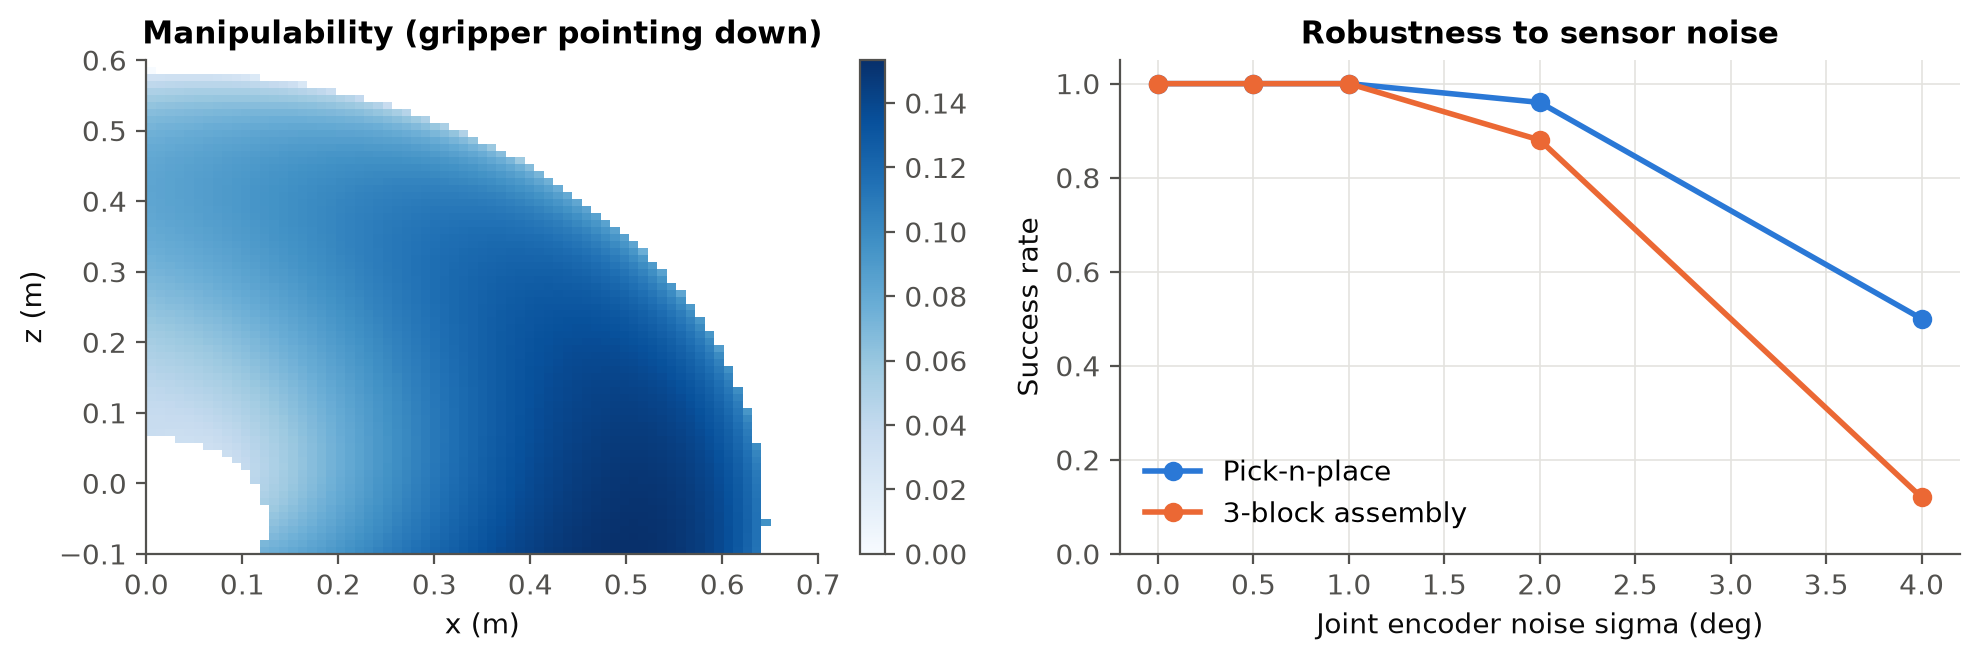
\includegraphics[width=0.95\linewidth]{manipulation_analysis.png}
\caption{Left: manipulability over the workspace. Right: success versus joint-sensor noise.}\label{fig:manip}\end{figure}

\section{Language understanding}
The language model detects 9 intents and labels the slots colour, object, source and destination. To test
generalisation fairly, the sentence templates were split into training and test sets before sentences were
generated. A fine-tuned DistilBERT teacher was distilled into a small student~\cite{jointbert,tinybert}
(Table~\ref{tab:nlu}, Figure~\ref{fig:nlu}).

\begin{table}[H]\centering\small\caption{Language understanding on unseen sentence patterns.}\label{tab:nlu}\fit{tab_nlu}\end{table}
\begin{figure}[H]\centering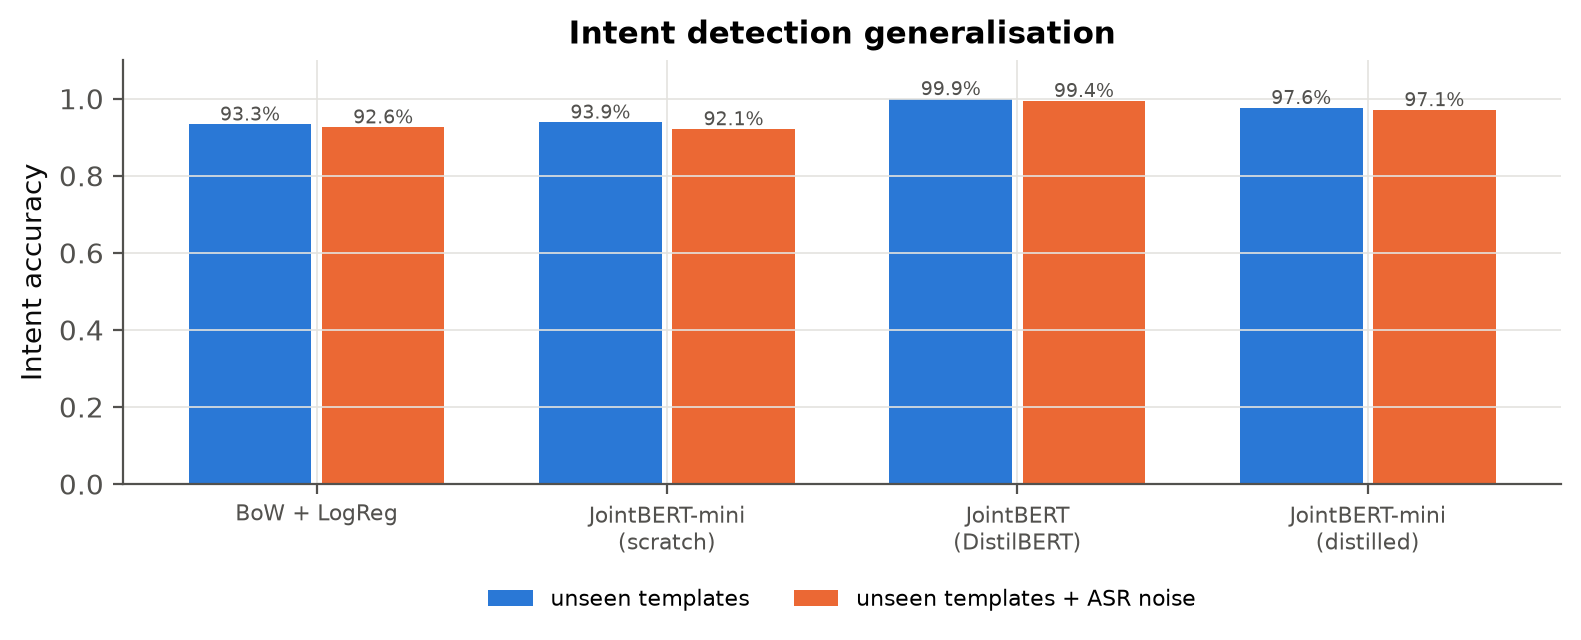
\includegraphics[width=0.95\linewidth]{nlu_comparison.png}
\caption{Intent accuracy of each language model.}\label{fig:nlu}\end{figure}

\section{Speech}
Speech is converted to text by Whisper-base~\cite{whisper} and replies are spoken by Piper, a VITS
model~\cite{vits}. On 150 held-out spoken commands the full pipeline was tested (Table~\ref{tab:voice}).

\begin{table}[H]\centering\small\caption{Results on 150 spoken test commands.}\label{tab:voice}\fit{tab_voice}\end{table}

\section{Edge deployment}
All networks were exported to ONNX and quantised to INT8 (Table~\ref{tab:edge}, Figure~\ref{fig:edge}). INT8 makes
the models 3--4$\times$ smaller with almost no accuracy loss for PPO and the language model. The image-based DQN is
more sensitive; calibrated static quantisation recovers most of its accuracy (Table~\ref{tab:dqnq}). Latency was
measured on a laptop CPU, not on a Jetson.

\begin{table}[H]\centering\small\caption{Model size and time per inference.}\label{tab:edge}\fit{tab_edge}\end{table}
\begin{table}[H]\centering\small\caption{INT8 quantisation of the image-based DQN.}\label{tab:dqnq}\fit{tab_dqn_quant}\end{table}
\begin{figure}[H]\centering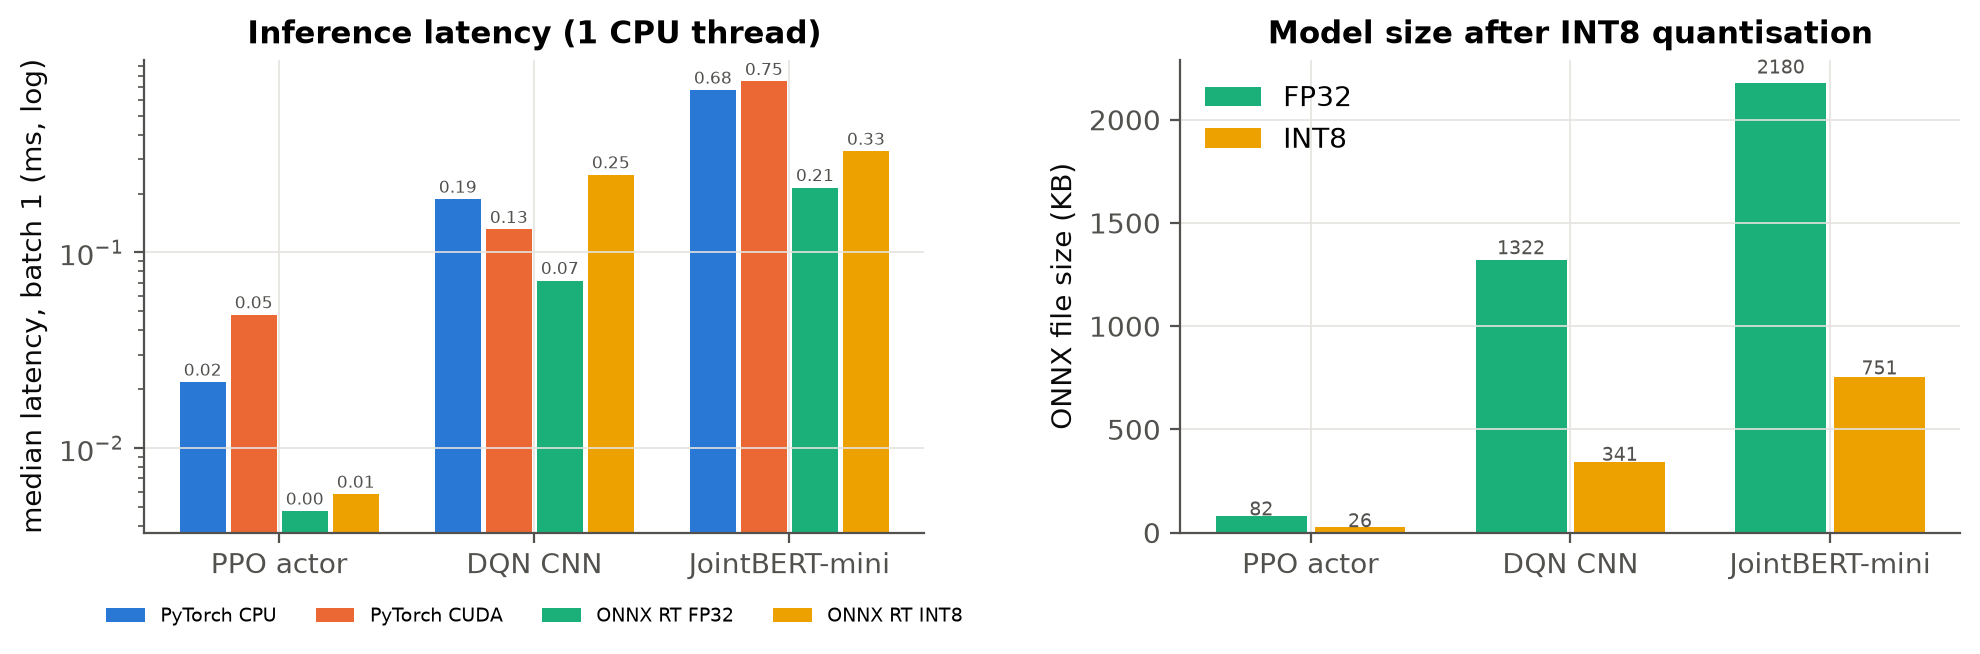
\includegraphics[width=\linewidth]{edge_benchmark.png}
\caption{Latency and model size of the exported models.}\label{fig:edge}\end{figure}

% =====================================================================
\chapter{Integrated System Demonstration}
\label{ch:demo}
The complete robot was run on a scripted eight-turn conversation using the shielded ONNX models
(Figure~\ref{fig:demo}, Table~\ref{tab:demo}). All six navigations succeeded without collision, and the arm completed
every pick, place and stacking task.

\begin{figure}[H]\centering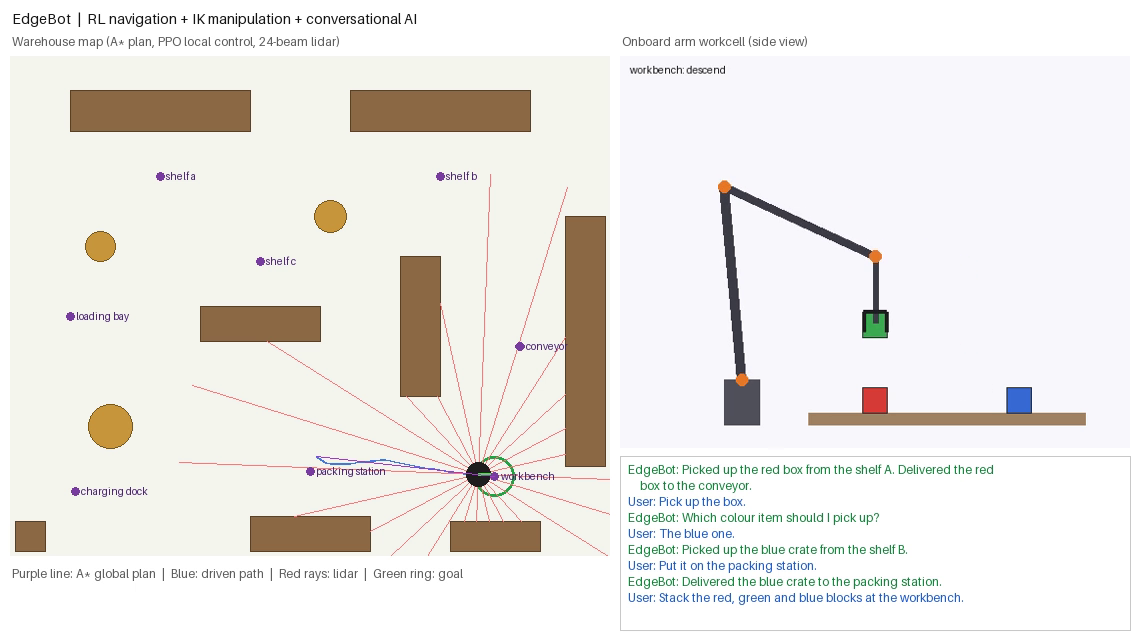
\includegraphics[width=\linewidth]{demo_frame.png}
\caption{Frame from the demonstration: warehouse map with the A* route (purple), the driven path (blue) and the lidar
beams (red), the arm workcell and the conversation.}\label{fig:demo}\end{figure}

\begin{table}[H]
\centering\small
\caption{Demonstration conversation.}
\label{tab:demo}
\begin{tabularx}{\linewidth}{lY}
\toprule
User command & Robot response \\
\midrule
hello jetbot & Greets the user. \\
move the red box from shelf a to the conveyor & Drives to shelf A, picks the red box, drives to the conveyor and delivers it. \\
pick up the box & Asks: ``Which colour item should I pick up?'' \\
the blue one & Completes the earlier request and picks the blue crate from shelf B. \\
put it on the packing station & Resolves ``it'' to the carried crate and delivers it. \\
stack the red green and blue blocks at the workbench & Builds the three-block tower. \\
what is your status & Reports location, load, battery and last task. \\
go back to the charging dock & Returns to the dock. \\
\bottomrule
\end{tabularx}
\end{table}

% =====================================================================
\chapter{Discussion}
\label{ch:discussion}

\section{How the project answers the open challenges of the survey}
Table~\ref{tab:challenges} maps the six open challenges identified by the 2025 survey~\cite{zhu2025survey} to the
parts of this project that address them.

\begin{table}[H]
\centering\small
\caption{Open challenges of the survey and how EdgeBot addresses them.}
\label{tab:challenges}
\begin{tabularx}{\linewidth}{lY}
\toprule
Survey challenge & How this project addresses it \\
\midrule
Adaptability in dynamic environments & Policy trained on a new random warehouse every episode; 96.0\% success on 300 unseen layouts. \\
Sensor noise and fusion & Robust shield keeps 0--1\% collisions under spurious and noisy lidar (novelty). \\
Multi-robot collaboration & Not addressed; listed as future work. \\
Sim-to-real transfer & Corruption model from a 2025 sim-to-real study; domain randomisation compared; ONNX/INT8 export ready for hardware. \\
Safety and explainability & Rule-based, transparent shield on top of the black-box policy; 0.0\% collisions for all FP32 and INT8 policies (novelty). \\
Cross-domain applications & Warehouse logistics with voice interaction; the shield is independent of the task and the policy. \\
\bottomrule
\end{tabularx}
\end{table}

\section{Why the shield is better than retraining}
Retraining with noise changes the policy so that it tolerates noise on average, but it does not give any guarantee
on an individual step, and it lowered both success and safety in this experiment. The shield instead checks every
single action against the physics of the robot and the current sensor data. It is independent of how the policy was
trained or compressed, so one shield protects all policies, and it adds no training cost.

\section{Lessons learned}
\begin{itemize}
\item A safety layer must itself be robust to bad sensor data; otherwise it can make the robot useless (3.0\%
success with the naive shield under corruption).
\item Simple, physics-based checks can outperform additional training for safety.
\item Use RL where the world is unknown (driving among random obstacles) and exact methods where it is known (arm
geometry).
\end{itemize}

% =====================================================================
\chapter{Conclusion and Future Work}
\label{ch:conclusion}

\section{Conclusion}
This project built EdgeBot, a voice-commanded warehouse robot whose navigation is learned with PPO, and proposed a
robust, map-free, training-free lidar safety shield as its main contribution. The shield removes collisions for PPO
and DQN policies in both FP32 and INT8 form on 300 unseen layouts, survives lidar corruption that freezes a naive
shield, and outperforms retraining with domain randomisation in both success and safety without any training cost.
The project also reproduced the classical tabular RL results, compared DQN with PPO, and tested the SimBa network.

\section{Limitations}
All experiments are in simulation; latency was measured on a laptop rather than a Jetson; speech was tested with
synthetic voices; SimBa and domain randomisation were run with one seed each; and the shield can miss obstacles
thinner than the gap between two lidar beams.

\section{Future work}
\begin{itemize}
\item Deploy the shielded INT8 policy on a physical JetBot with a Jetson board.
\item Extend the shield to moving obstacles by predicting their motion from consecutive scans.
\item Use a denser lidar and an adaptive margin based on speed.
\item Extend to multiple robots sharing the same warehouse.
\end{itemize}

% =====================================================================
\begin{thebibliography}{99}
\bibitem{sutton} R.~S.~Sutton and A.~G.~Barto, \emph{Reinforcement Learning: An Introduction}, 2nd ed., MIT Press, 2018.
\bibitem{dqn} V.~Mnih et al., ``Human-level control through deep reinforcement learning,'' \emph{Nature}, vol.~518, 2015.
\bibitem{ddqn} H.~van Hasselt, A.~Guez and D.~Silver, ``Deep reinforcement learning with double Q-learning,'' AAAI, 2016.
\bibitem{ppo} J.~Schulman et al., ``Proximal policy optimization algorithms,'' arXiv:1707.06347, 2017.
\bibitem{gae} J.~Schulman et al., ``High-dimensional continuous control using generalized advantage estimation,'' ICLR, 2016.
\bibitem{zhu2025survey} Y.~Zhu, W.~Z.~W.~Hasan, H.~R.~H.~Ramli, N.~M.~H.~Norsahperi, M.~S.~M.~Kassim and Y.~Yao, ``Deep reinforcement learning of mobile robot navigation in dynamic environment: a review,'' \emph{Sensors}, vol.~25, no.~11, 3394, 2025.
\bibitem{alshiekh} M.~Alshiekh et al., ``Safe reinforcement learning via shielding,'' AAAI, 2018.
\bibitem{realizable2024} ``Realizable continuous-space shields for safe reinforcement learning,'' arXiv:2410.02038, 2024.
\bibitem{reasan2025} ``REASAN: Learning reactive safe navigation for legged robots,'' arXiv:2512.09537, 2025.
\bibitem{uavsafe2026} ``Lightweight safe reinforcement learning for end-to-end UAV navigation,'' arXiv:2607.01794, 2026.
\bibitem{quarl} S.~Krishnan et al., ``QuaRL: Quantization for fast and environmentally sustainable reinforcement learning,'' TMLR, 2022.
\bibitem{quantprune2024} ``The impact of quantization and pruning on deep reinforcement learning models,'' arXiv:2407.04803, 2024.
\bibitem{quantctrl2025} ``Learning quantized continuous controllers for integer hardware,'' arXiv:2511.07046, 2025.
\bibitem{edgesurvey2026} ``Embodied foundation models at the edge: a survey of deployment constraints and mitigation strategies,'' arXiv:2603.16952, 2026.
\bibitem{omni2025} Z.~Wang et al., ``Omni-Perception: Omnidirectional collision avoidance for legged locomotion in dynamic environments,'' arXiv:2505.19214, 2025.
\bibitem{sim2real2025} ``Sim-to-real transfer for mobile robots with reinforcement learning: from NVIDIA Isaac Sim to Gazebo and real ROS 2 robots,'' arXiv:2501.02902, 2025.
\bibitem{sim2realsurvey2025} ``A survey of sim-to-real methods in RL: progress, prospects and challenges with foundation models,'' arXiv:2502.13187, 2025.
\bibitem{navrlpp2026} ``NavRL++: A system-level framework for improving sim-to-real transfer in reinforcement learning-based robot navigation,'' arXiv:2605.15559, 2026.
\bibitem{simba2025} H.~Lee et al., ``SimBa: Simplicity bias for scaling up parameters in deep reinforcement learning,'' ICLR, 2025 (arXiv:2410.09754).
\bibitem{jointbert} Q.~Chen, Z.~Zhuo and W.~Wang, ``BERT for joint intent classification and slot filling,'' arXiv:1902.10909, 2019.
\bibitem{tinybert} X.~Jiao et al., ``TinyBERT: Distilling BERT for natural language understanding,'' Findings of EMNLP, 2020.
\bibitem{whisper} A.~Radford et al., ``Robust speech recognition via large-scale weak supervision,'' ICML, 2023.
\bibitem{vits} J.~Kim, J.~Kong and J.~Son, ``Conditional variational autoencoder with adversarial learning for end-to-end text-to-speech,'' ICML, 2021.
\end{thebibliography}

% =====================================================================
\appendix
\titleformat{\chapter}[display]{\normalfont\Large\bfseries}{\large Appendix \thechapter}{4pt}{\LARGE}
\chapter{Anticipated Questions}
\label{app:qa}
The following questions are based on the open challenges of the 2025 survey~\cite{zhu2025survey} and on the
contributions of this project.

\begin{description}[style=nextline,leftmargin=0pt,itemsep=6pt]
\item[What is the novelty of the project?] A robust, map-free, training-free lidar safety shield that removes
collisions for FP32 and INT8 policies and survives faulty lidar readings, evaluated inside a complete
voice-commanded robot.
\item[How is it better than existing shields?] Existing shields need a formal model or map, or are learned
networks, and are tested on full-precision policies. This shield needs none of these and is tested on INT8 policies
and corrupted lidar (Table~\ref{tab:gap}).
\item[How is it better than retraining with noise?] On corrupted lidar it gives 95.0\% success and 0.0\% collisions
(INT8 PPO) versus 89.3\% and 7.0\% for the domain-randomised policy, with no training (Table~\ref{tab:compare}).
\item[Why did the first shield fail under corruption?] It treated spurious short readings as real obstacles and
froze the robot (3.0\% success). The median filter removes single-beam spikes.
\item[Why not just train a safer policy?] Training improves average behaviour but gives no per-step check, must be
repeated for each new or quantised policy, and in this project lowered performance.
\item[Why PPO and not DQN?] PPO reached 96.0\% success against 86.0\% for DQN, uses continuous actions and trains
stably.
\item[How do you know the policy generalises?] Every training episode uses a new random warehouse and testing uses
300 layouts from seeds never seen in training.
\item[What does the survey say is missing in the field?] Safety, robustness to sensor noise, sim-to-real transfer
and explainability; this project addresses safety and sensor noise directly (Table~\ref{tab:challenges}).
\item[What is the difference between SARSA and Q-learning in your results?] Q-learning learns the shortest, risky
path; SARSA learns a safer path because it accounts for its own exploration.
\item[What are the limitations?] Simulation only, laptop latency, synthetic speech, one seed for SimBa and domain
randomisation, and very thin obstacles between beams.
\end{description}

\chapter{Reproducing the Results}
\label{app:repro}
All code, trained models and results are available at \url{https://github.com/MrMehulkhanna/edgebot}.
\begin{center}
\small
\begin{tabular}{ll}
\toprule
Step & Command \\
\midrule
Run the tests & \texttt{python -m pytest -q} \\
Tabular RL & \texttt{python scripts/run\_tabular.py} \\
Train PPO & \texttt{python scripts/train\_nav\_ppo.py --steps 5000000} \\
Train DQN & \texttt{python scripts/train\_nav\_dqn.py --obs lidar} \\
Shield experiment & \texttt{python scripts/eval\_shield.py} \\
Robustness experiment & \texttt{python scripts/eval\_robustness.py} \\
Live demo & \texttt{python scripts/run\_demo.py --interactive} \\
Web control panel & \texttt{python scripts/web\_app.py} \\
\bottomrule
\end{tabular}
\end{center}

\end{document}
